%! Author = anton
%! Date = 31/08/2024

\subsection{Calibration Consideration On Selected Models}
\label{subsec:bestModels}
\textbf{Best Models}

Taking the best configurations of each method we have:
\begin{itemize}
    \item \textbf{Logistic Regression}: \(\lambda=3.162*10^{-2}\), minDCF is 0.2436 and actDCF is 0.4972
    \item \textbf{Support Vector Machine}: with RBF Kernel with \(\gamma=0.1\) and \(C=100\), minDCF is 0.1845 and actDCF is 0.3581
    \item \textbf{Gaussian Mixture Model}: with Diagonal convolution and \((nc0=8, nc1=32)\) where \(nc0\) is the number of
    component for class 0 and \(nc1\) is number of component for class 1, minDCF is 0.1312 and actDCF is 0.1517
\end{itemize}

In \autoref{fig:BestConfiguration} we see the behaviour of the 3 best models we have selected, now we will apply the calibration to these.

\begin{figure}[h!]
    \centering
    \begin{subfigure}[b]{0.30\linewidth}
        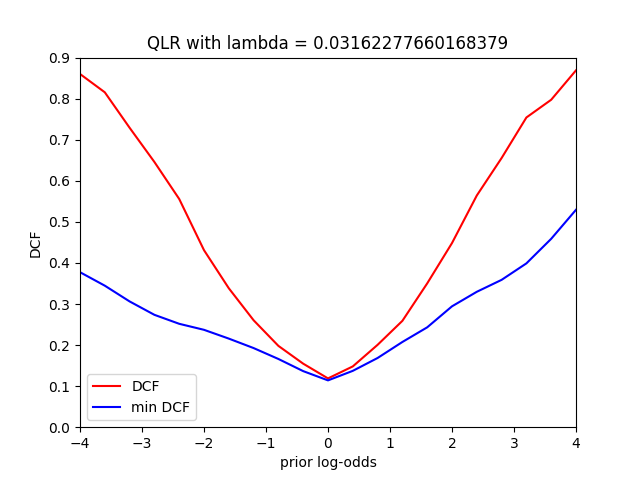
\includegraphics[width=\linewidth]{Lab/11. Lab 11/Images/BestConfiguration/01. QLR}
        \label{fig:QLRBest}
    \end{subfigure}
    \begin{subfigure}[b]{0.30\linewidth}
        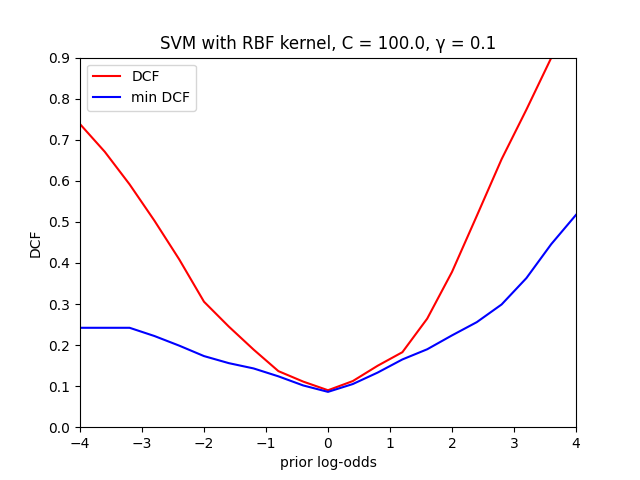
\includegraphics[width=\linewidth]{Lab/11. Lab 11/Images/BestConfiguration/02. SVM}
        \label{fig:SVM}
    \end{subfigure}
    \begin{subfigure}[b]{0.30\linewidth}
        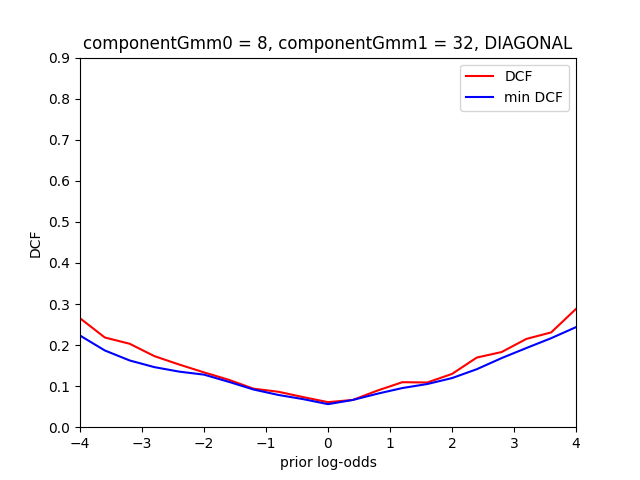
\includegraphics[width=\linewidth]{Lab/11. Lab 11/Images/BestConfiguration/03. GMM}
        \label{fig:GMM}
    \end{subfigure}
    \caption{Shows minDCF and actDCF for three best models}
    \label{fig:BestConfiguration}
\end{figure}

\subsection{Calibration Scores For Best Models}
\label{subsec:calibrationScores}

\begin{figure}[h!]
    \centering
    \begin{subfigure}[b]{0.40\linewidth}
        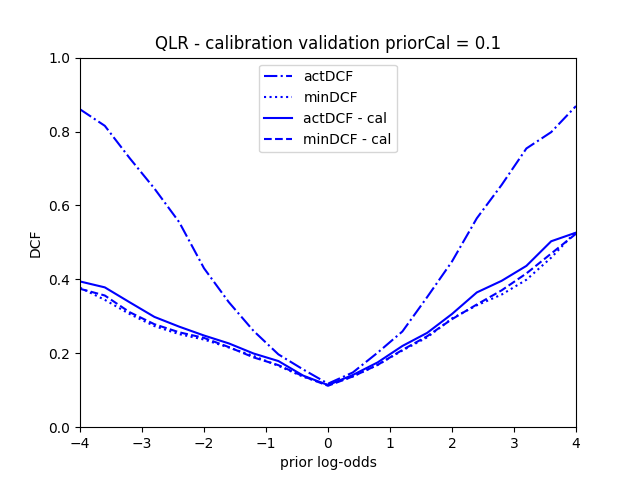
\includegraphics[width=\linewidth]{Lab/11. Lab 11/Images/CalibrationAndFusion/01. QLR}
        \label{fig:QLRCalibration}
    \end{subfigure}
    \begin{subfigure}[b]{0.40\linewidth}
        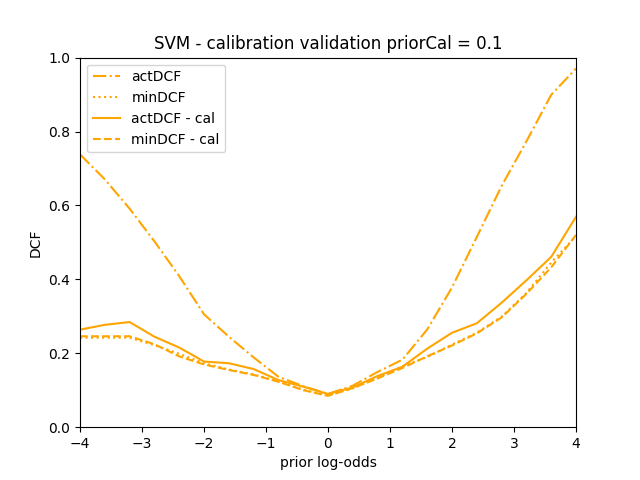
\includegraphics[width=\linewidth]{Lab/11. Lab 11/Images/CalibrationAndFusion/02. SVM}
        \label{fig:SVMCalibration}
    \end{subfigure}
    \begin{subfigure}[b]{0.40\linewidth}
        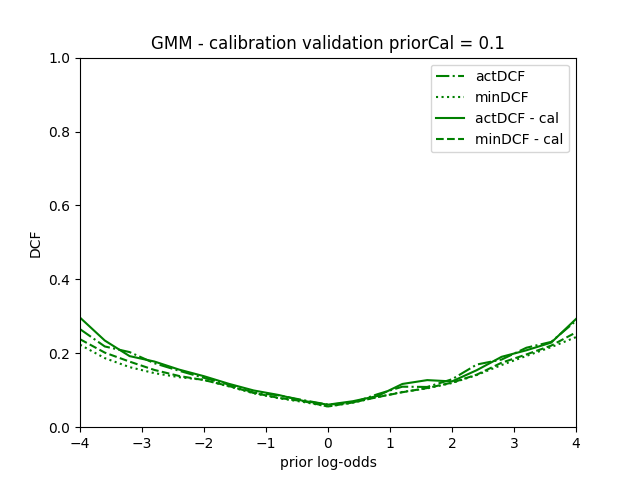
\includegraphics[width=\linewidth]{Lab/11. Lab 11/Images/CalibrationAndFusion/03. GMM}
        \label{fig:GMMCalibration}
    \end{subfigure}
    \begin{subfigure}[b]{0.40\linewidth}
        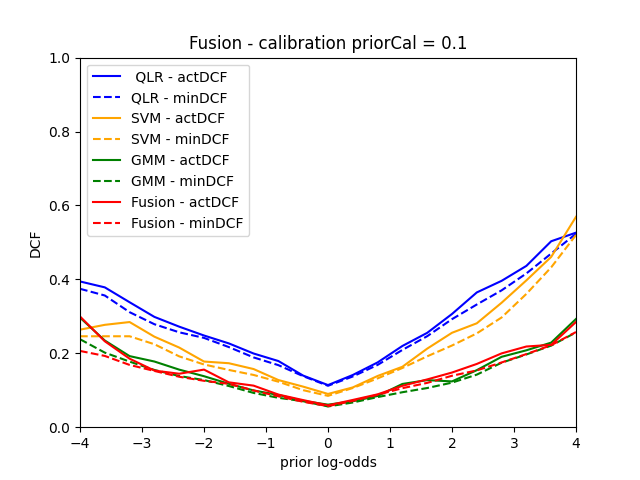
\includegraphics[width=\linewidth]{Lab/11. Lab 11/Images/CalibrationAndFusion/04. Fusion}
        \label{fig:FusionCalibration}
    \end{subfigure}
    \caption{Shows result of each model before and after calibration}
    \label{fig:BestConfigurationCalibration}
\end{figure}


\begin{table}[h!]
    \centering
    \begin{tabular}{>{\centering\arraybackslash}p{2.9cm} >{\centering\arraybackslash}p{2.9cm} >{\centering\arraybackslash}p{2.9cm} >{\centering\arraybackslash}p{2.9cm}}
        \toprule
        & \multicolumn{3}{c}{\textbf{Uncalibrated Models [minDCF - actDCF]}} \\
        \midrule
        \textbf{QLR} & \multicolumn{3}{c}{0.2436 - 0.4972} \\
        \textbf{SVM} & \multicolumn{3}{c}{0.1845 - 0.3581} \\
        \textbf{GMM} & \multicolumn{3}{c}{0.1312 - 0.1517} \\
        \midrule
        \midrule
        & \multicolumn{3}{c}{\textbf{Calibrated Models [minDCF - actDCF]}} \\
        \midrule
        & \(\tilde{\pi} = 0.1\) & \(\tilde{\pi} = 0.5\) & \(\tilde{\pi} = 0.9\) \\
        \midrule
        \textbf{QLR}    & 0.2486 - 0.2721       & 0.2496 - 0.2609       & 0.2480 - 0.2657       \\
        \textbf{SVM}    & 0.1794 - 0.1894       & 0.1814 - 0.2032       & 0.1881 - 0.2020       \\
        \textbf{GMM}    & 0.1324 - 0.1518       & 0.1314 - 0.1518       & 0.1283 - 0.1559       \\
        \midrule
        \textbf{Fusion} & 0.1304 - 0.1568       & 0.1373 - 0.1639       & 0.1382 - 0.1731       \\
        \bottomrule
    \end{tabular}
    \captionsetup{justification=justified,singlelinecheck=false,format=hang}
    \caption{Show minDCF and actDCF for different models before and after calibration}
    \label{tab:resultUnCalibratedAndCalibratedModels}
\end{table}
%
%
%\begin{table}[h!]
%    \centering
%    \begin{tabular}{>{\centering\arraybackslash}p{2.9cm} >{\centering\arraybackslash}p{2.9cm} >{\centering\arraybackslash}p{2.9cm} >{\centering\arraybackslash}p{2.9cm}}
%        \toprule
%        & \multicolumn{3}{c}{\textbf{Uncalibrated Models [minDCF - actDCF]}} \\
%        \midrule
%        \textbf{QLR} & \multicolumn{3}{c}{} \\
%        \textbf{SVM} & \multicolumn{3}{c}{} \\
%        \textbf{GMM} & \multicolumn{3}{c}{} \\
%        \midrule
%        \midrule
%        & \multicolumn{3}{c}{\textbf{Calibrated Models [minDCF - actDCF]}} \\
%        \midrule
%        & \(\tilde{\pi} = 0.1\) & \(\tilde{\pi} = 0.5\) & \(\tilde{\pi} = 0.9\) \\
%        \midrule
%        \textbf{QLR}    &                       &                       &                       \\
%        \textbf{SVM}    &                       &                       &                       \\
%        \textbf{GMM}    &                       &                       &                       \\
%        \midrule
%        \textbf{Fusion} &                       &                       &                       \\
%        \bottomrule
%    \end{tabular}
%    \captionsetup{justification=justified,singlelinecheck=false,format=hang}
%    \caption{Show minDCF and actDCF for different models before and after calibration on eval dataset}
%    \label{tab:resultUnCalibratedAndCalibratedModelsOnEval}
%\end{table}